%%%%%
%%%%% Chapter 3
%%%%%
\chapter{Simple Sampling of Probability distributions Using Random numbers}
This Chapter is devoted to the following question: How can we 
generate sequences of random numbers which are distributed 
according to some given distribution?

A simple answer to this question would be to exploit some 
intrinsically random physical process. For example, one could 
record a sequence of the decay times of some radioactive substance 
and use this truly random sequence of numbers in a Monte--Carlo
simulation. Although tables of millions of such true random 
numbers exist in practice this approach turns out to be very
impractical. Monte--Carlo simulations need very long sequences of 
random numbers, so that we have to find more efficient ways to 
generate them. This requirement is satisfied 
by so--called pseudo--random numbers.
Pseudo--random numbers are generated numerically with the help of 
some simple algorithm on some computer. Consequently, they are
reproducible. This is, however, not a drawback. In fact, the 
reproducibility may be very useful if we want to check our 
simulation algorithms. 

Pseudo--random numbers are, the name already underlines it, not 
truly random. However, their statistical properties are very 
similar to the statistical properties of truly random numbers. So, 
for all practical purposes pseudo--random numbers appear to be 
random. Let us now see how such pseudo--random numbers can be 
generated.

\section{The generation of uniformly distributed random numbers}
We will begin with the generation of uniformly distributed random 
numbers on the interval $[0,1)$. In the following we will often 
omit the prefix pseudo. 

The best known algorithm for the generation of uniformly 
distributed random numbers is the linear congruential method, 
which given an initial integer "seed" value $I_1$ produces random 
integers recursively using the formula
\begin{equation*}
I_{n+1} = (aI_n +c) \mod M,
\end{equation*}
where $a$, $c$, and $M$ are integer constants which have to be 
chosen appropriately. 
The randomness of the above algorithm results from the fact that 
after some multiplications with $a$ the result exceeds $M$ and is 
consequently truncated. Since the integers $I_n$ lie between 1 and 
$M$ a random number $R$ uniformly distributed 
between 0 and 1 is obtained as
\begin{equation*}
R = \frac{I_n}{M}.
\end{equation*}
Unfortunately, MATLAB does not have integer arithmetic so the above algorithm 
has to be implemented using the {\sf rem} (remainder) function 
instead of the modulo function. A corresponding code could be
\begin{verbatim}
I(n+1) = floor( rem(a*I(n) + c,M) ).
\end{verbatim}
The MATLAB function {\sf floor} rounds towards minus infinity.
In order to get familiar with this algorithm we want to generate a 
sequence of pseudo--random numbers for the following parameters:
we choose the multiplier to be $a=5$, the increment $c=3$, and the 
modulo $M=8$. Obviously the longest period of random numbers will
have the length 8. The generation of the random sequences will
be achieved with the program {\sf trandom1}.

\subsubsection{Listing of the program trandom1.m}
\inputlisting{./Listings/trandom1.m}

Run with the above parameters the program generates the sequence
\begin{equation*}
1, 0, 3, 2, 5, 4, 7, 6, 1, 0, 3, 2 \ldots
\end{equation*}
which has also been plotted in Fig. (\ref{F_TRANDOM1}).
\begin{figure}
\label{F_TRANDOM1}
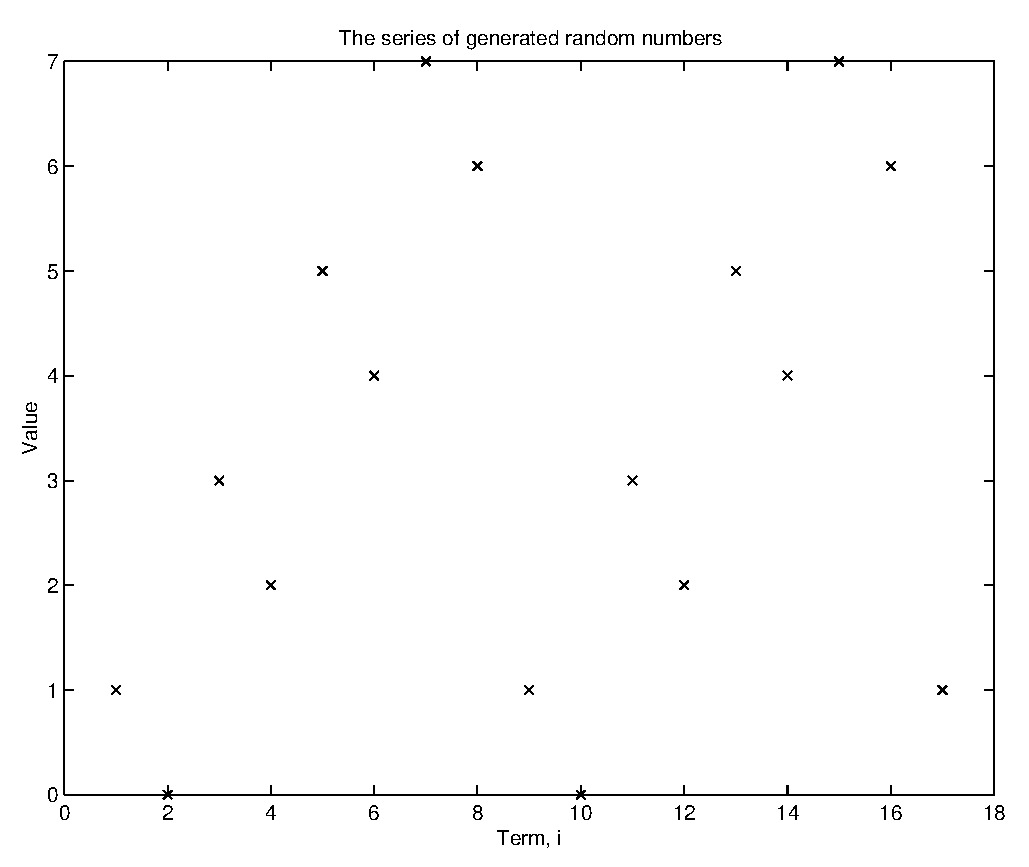
\includegraphics[width=10cm]{./Figures/f_trandom1.eps}
\caption{Successive values in a series of random numbers generated
for a=5, c=3, M=8. Note that the even numbers are always one less 
then the odd ones!}
\end{figure}
It might be instructive to run the program keeping the multiplier $a$ 
and the modulo $M$ fixed while changing the increment $c$. The result of 
these runs are summarized in Table \ref{T_LCG}.

\begin{table}
\label{T_LCG}
\caption{Series of random numbers for the linear congruential 
generator of the form $I_{n+1} = (5I_n +c) \mod 8$}
\begin{center}
\begin{tabular}{ccc} \hline\hline
c &  $I_n$ & Period  \\ \hline
1 & 1,6,7,4,5,2,3,0 & 8 \\
2 & 1,7,5,3,1,7,5,3 & 4 \\
  & 4,6,0,2,4,6,0,2 & 4 \\
3 & 1,0,3,2,5,4,7,6 & 8 \\
4 & 1,1,1,1,1,1,1,1 & 1 \\
  & 2,6,2,6,2,6,2,6 & 2 \\
  & 3,3,3,3,3,3,3,3 & 1 \\
  & 4,0,4,0,4,0,4,0 & 2 \\
  & 5,5,5,5,5,5,5,5 & 1 \\
  & 7,7,7,7,7,7,7,7 & 1 \\
5 & 1,2,7,0,5,6,3,4 & 1 \\
6 & 1,3,5,7,1,3,5,7 & 4 \\
  & 2,0,6,4,2,0,6,4 & 4 \\
7 & 1,4,3,6,5,0,7,2 & 8 \\ \hline \hline
\end{tabular}
\end{center}
\end{table}
It is evident that a wrong  choice of the constants leads to a 
very poor random sequence.

It can be shown \cite{Knuth}  that in the case $c=0$ the full 
period, 1 to $M-1$ can be achieved by choosing $M$ as a prime 
number and for $a$, a primitive element modulo $m$, i.e., for all 
prime divisors, $p$, of $(M-1)$, 
\begin{equation*}
a^{(M-1)/p} \quad {\rm mod} \quad M \ne 1.
\end{equation*}
For the case of $c\ne 0$ the full period is obtained if the 
following three conditions are satisfied:

(i) $c$ and $M$ are relatively prime,

(ii) $a \quad {\rm mod} \quad p = 1$ for each prime factor $p$ of $M$,

(iii) $a \quad {\rm mod} \quad 4 = 1$ if 4 divides $M$.

It is evident that the greater the modulus the longer the period.
For example the MATLAB random number generating function uses
\begin{equation*}
a= 16807; c=0; M=2^{31}-1.
\end{equation*}
to generate equally distributed random numbers in the interval
$[0,1]$
This chioce has been suggested by Park and Miller \cite{PRESS}.
The period of the generator is $2^{31}-2 \approx 2.1 \times 10^9$.
Another popular random number generator uses
\begin{equation*}
a= 65539; M=2^{31}-1; c=0,
\end{equation*}
and will be used in the following program {\sf trandom2.m}. There 
we will draw 3000 random numbers using the linear 
congruential method. In the program we will check the quality of 
the generator by plotting the 1D, 2D, and 3D distribution of the 
pseudo--random numbers. The results of the test can be seen in 
Figs. (\ref{F_TRANDOM2_1}), (\ref{F_TRANDOM2_2}), 
(\ref{F_TRANDOM2_3}), and (\ref{F_TRANDOM2_4}).

\subsubsection{Listing of the program trandom2.m}
\inputlisting{./Listings/trandom2.m}

\subsubsection{Listing of the function {\sf random1}}
\inputlisting{./Listings/random1.m}

\begin{figure}
\label{F_TRANDOM2_1}
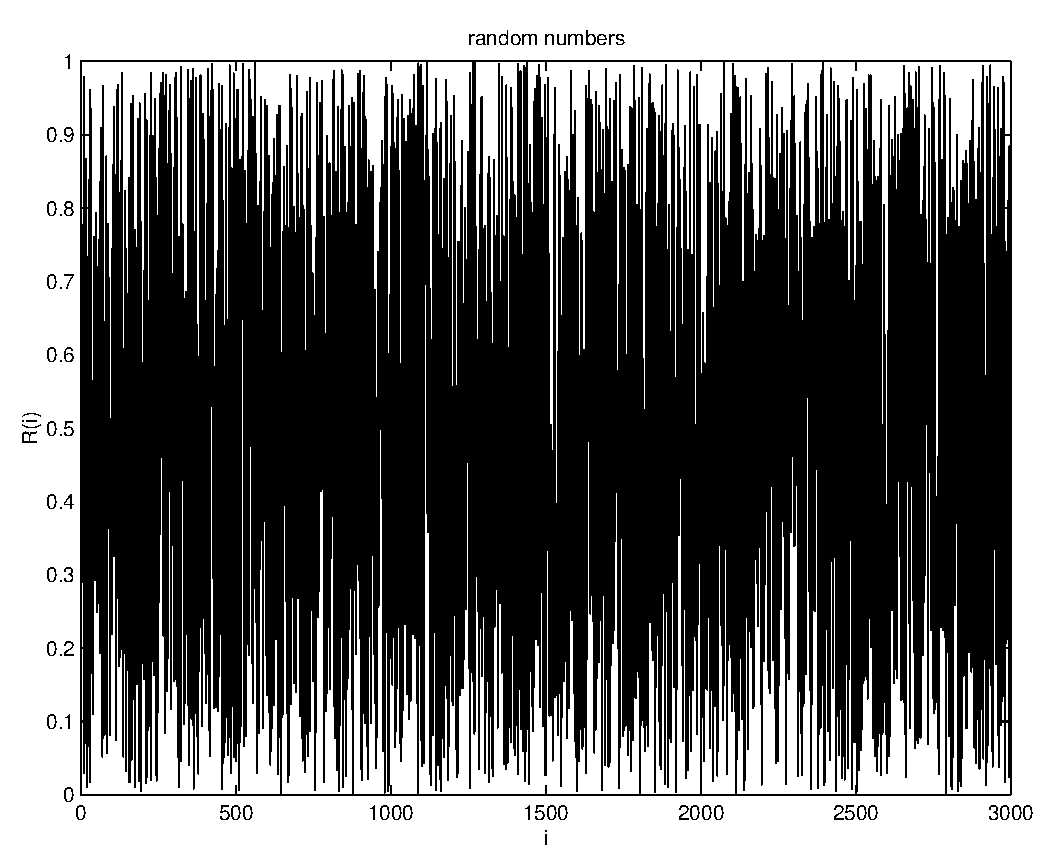
\includegraphics[width=10cm]{./Figures/f_trandom2_1.eps}
\caption{Successive values in a series of 3000 random numbers generated
for $a=65539$, $c=0$, $M=2^{31}-1$.}
\end{figure}

\begin{figure}
\label{F_TRANDOM2_2}
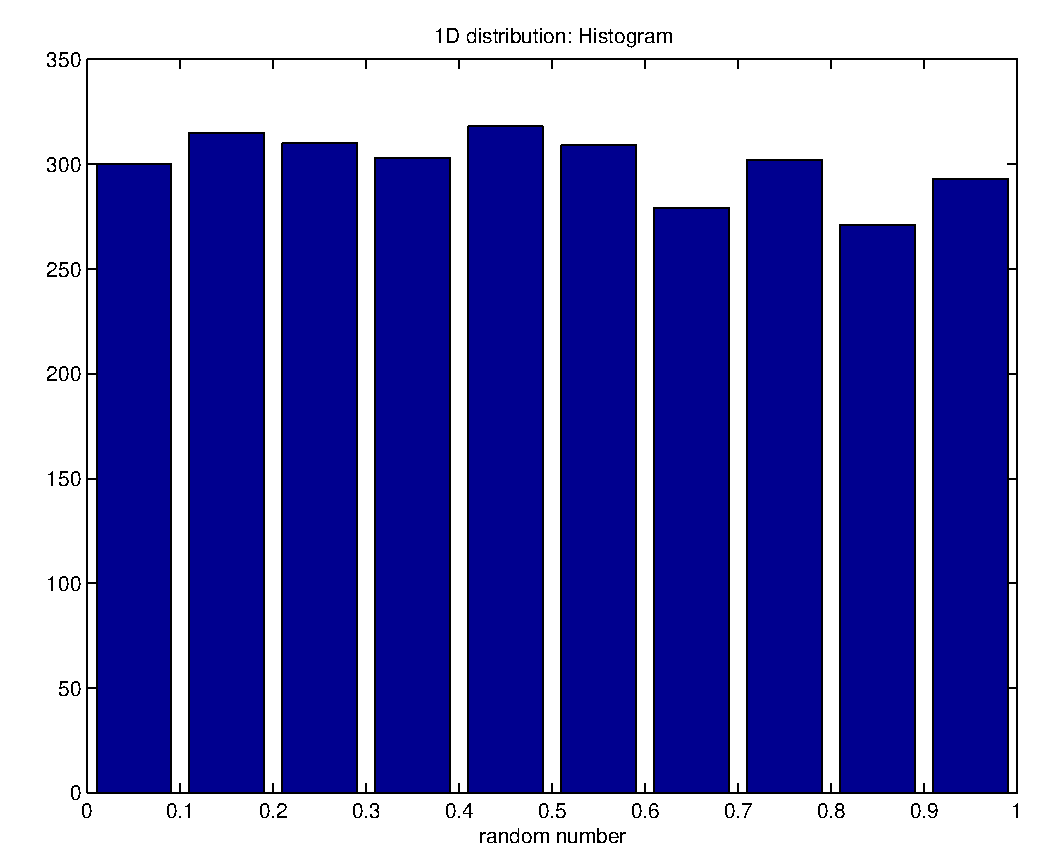
\includegraphics[width=10cm]{./Figures/f_trandom2_2.eps}
\caption{Histogram for a series of 3000 random numbers generated
for $a=65539$, $c=0$, $M=2^{31}-1$.}
\end{figure}

\begin{figure}
\label{F_TRANDOM2_3}
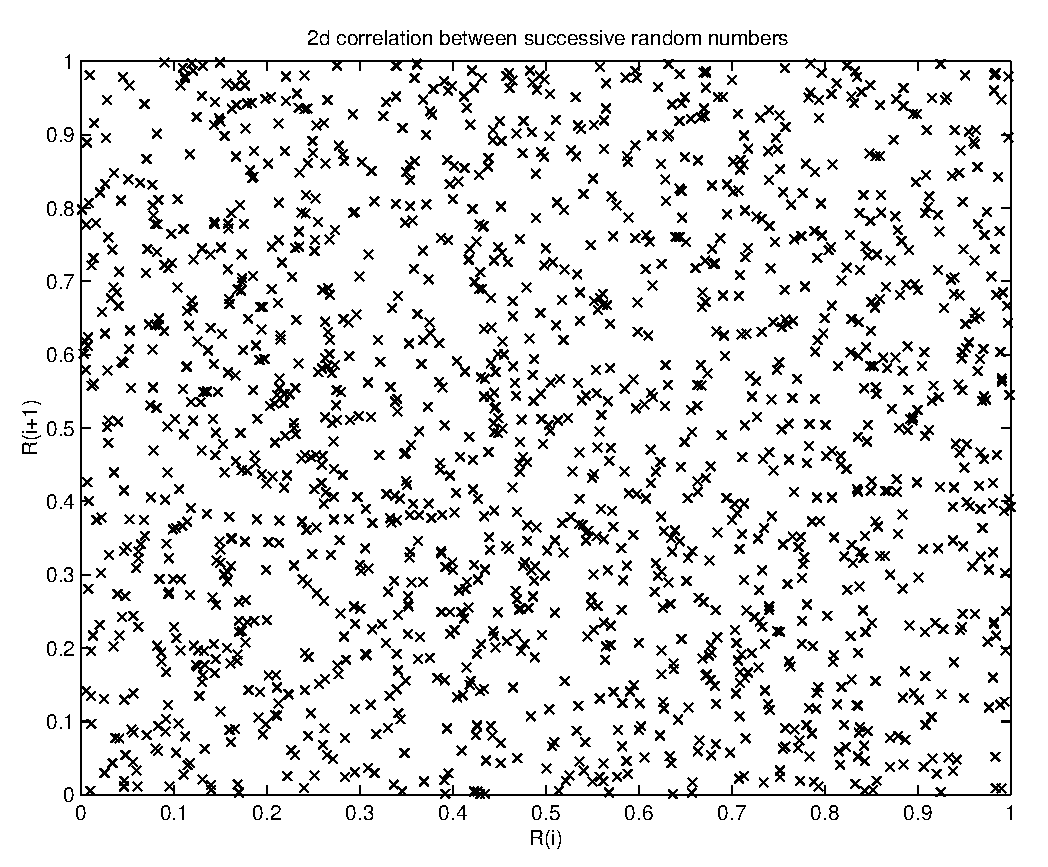
\includegraphics[width=10cm]{./Figures/f_trandom2_3.eps}
\caption{Correlation between successive values in a series of 3000 
random numbers generated for $a=65539$, $c=0$, $M=2^{31}-1$.}
\end{figure}


\begin{figure}
\label{F_TRANDOM2_4}
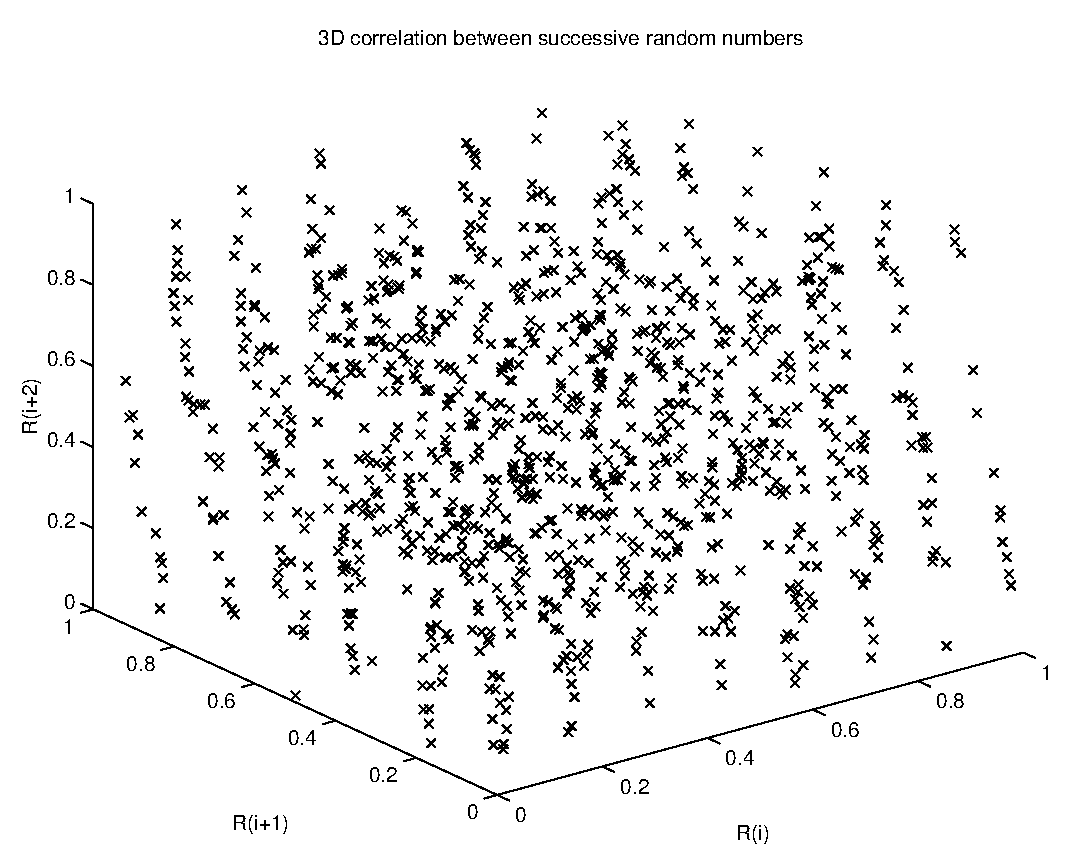
\includegraphics[width=10cm]{./Figures/f_trandom2_4.eps}
\caption{Correlation between successive values 
$R(i),R(i+1), R(i+2)$ in a series of 3000 random numbers generated
for $a=65539, c=0, M=2^{31}-1$.}
\end{figure}

The figures clearly reveal that the generator is not perfect.
In the exercise we will learn that choosing $a=16807$, the minimal
standard generator, 
significantly improves the performance. The performance of 
this minimal standard generator can be increased by shuffling
the output to remove low--order serial correlations (EXERCISE!!!!)
({\sf ran1} of Numerical Recipes).

In the book by Press et al. other "Quick and Dirty" linear 
congruential generators
are presented. Furthemore, it is important to remark 
that serial correlations can be broken up by 
combining two linear congruential generators.

There are also other algorithms for the generation of random 
numbers: Shift--register generators (Lit: Kirkpatrick and Stoll), 
Fibonacci generators (lit: Knuth, James) or quasi--random numbers 
and we refer the reader to the original literature. Special random
number generators for parallel computers has been developed.

\section{The Transfomation method: Invertible distributions}
In the previous section we have learned how to generate random 
numbers with a uniform probability distribution, so that the 
probability $p(x)dx$ to generate a random number between $x$ and $x+dx$
is given by
\begin{equation*}
p(x)dx = \left\{ \begin{array}{ll}
                   dx & 0<x<1 \\
                   0   & {\rm otherwise}.
                  \end{array}
         \right.
\end{equation*}
With the help of the random variable transformation theorem it is easy
to transform uniform deviates into random numbers which are 
distributed according to invertible, one--to--one, distributions.
We know from Chap. 2 that if we take a uniform deviate $x$ and then 
transform it to a new variable $y(x)$ the probability distribution
of $y$ is given by
\begin{equation}
p(y) = p(x) \left| \frac{dx}{dy}\right|.
\end{equation}
We want to derive a transformation which generates random numbers 
which are distributed according to a given
$p(y)$. Since $x$ is uniformly distributed the 
above equation reduces to
\begin{equation}
\label{INVERTIBLE}
\frac{dx}{dy} = p(y),
\end{equation}
which can be easily integrated
\begin{equation*}
x(y) = P(y) = \int^y p(y')dy'.
\end{equation*}
Hence, the transformation we are looking for is given by the 
inverse of $P(y)$. Thus, a random variable $Y$ with density $p(y)$
can be generated by uniform deviates through
\begin{equation*}
Y = Y(X) = P^{-1}(X).
\end{equation*}
In the following we will apply this method to generate 
exponentially and Gaussian distributed random numbers.

\subsection{Exponential distribution}
Let $p(y)= w\exp(-wy)$ for positive $y$. It follows from Eq. (\ref{INVERTIBLE})
that
\begin{equation*}
\frac{dx}{dy} = w \exp(-wy).
\end{equation*}
Therefore we get immediately
\begin{equation*}
x(y) = \int_0^{\infty} dy'w\exp(-wy') = 1-\exp(-wy).
\end{equation*}
The above expression is easily inverted
\begin{equation*}
y=-\frac{1}{w}\ln(1-x),
\end{equation*}
and since $x$ is equally distributed in $[0,1]$ we can generate 
exponentially distributed random numbers with the help of the 
formula
\begin{equation}
y = - \frac{1}{w} \ln(x).
\end{equation}
It is clear that in MATLAB such an exponentially distributed 
random number $Y$ can be generated with the help of the following 
line of code
\begin{verbatim}
y = - log( rand(1) )/w
\end{verbatim}
With the help of the simple program {\sf expdistr} we want to 
generate 1000 exponentially distributed random numbers and compare
them with the prescribed distribution. We check also the mean 
value and variance and compare them with the analytical expectation 
values.

\subsubsection{Listing of the program expdistr.m}
\inputlisting{./Listings/expdistr.m}

In Fig. (\ref{F_EXPDISTR}) we see the histogram of 1000 drawn exponentially 
distributed random numbers.
\begin{figure}
\label{F_EXPDISTR}
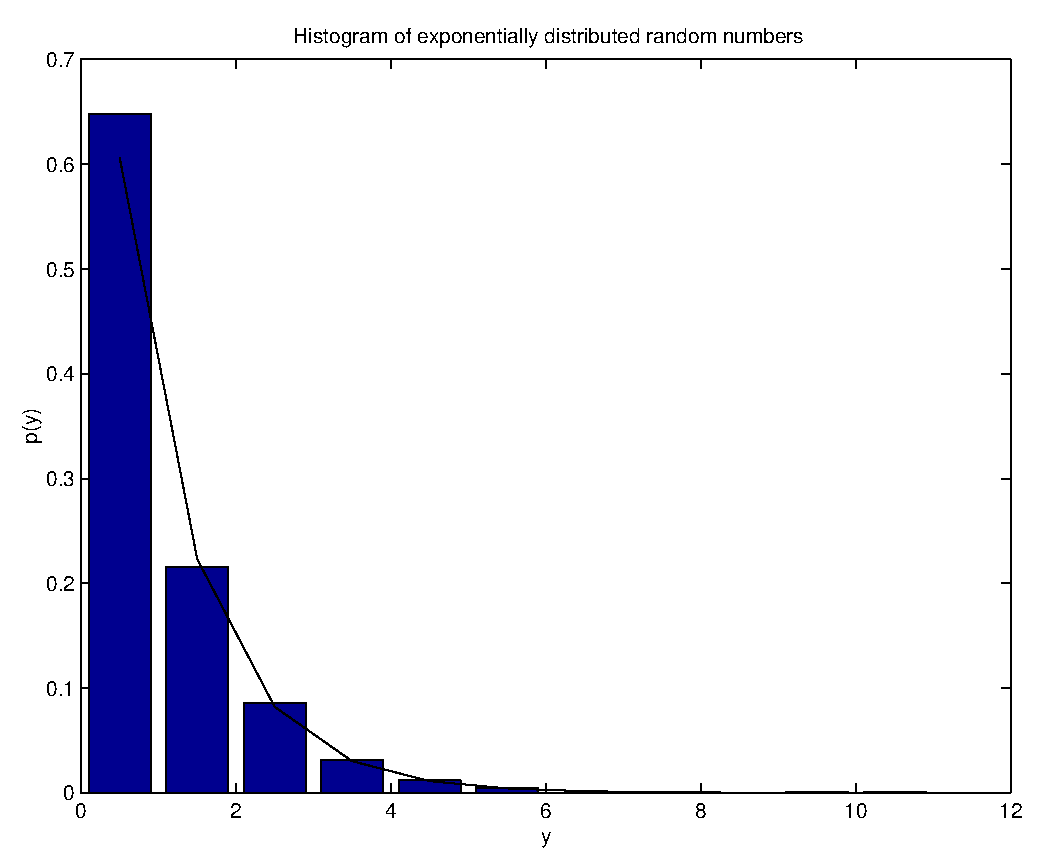
\includegraphics[width=10cm]{./Figures/f_expdistr.eps}
\caption{Histogram of 1000 exponentially distributed random numbers with
mean 1 generated according to the transformation method. The continuous
line represents the expected exponential distribution.}
\end{figure}

\subsection{Gaussian distributed random numbers}
Gaussian distributed random numbers can be obtained with the help 
of the multidimensional random variable transformation theorem.
Let us consider the transformation
\begin{eqnarray}
\label{GAUSS-GEN1}
y_1 & = & \sqrt{-2\log(x_1)} \cos(2 \pi x_2) \\
\label{GAUSS-GEN2}
y_2 & = & \sqrt{-2\log(x_1)} \sin(2 \pi x_2),
\end{eqnarray}
where $X_1$ and $X_2$ are uniformly distributed random numbers on 
the interval $[0,1]$. Equivalently we can write
\begin{eqnarray*}
x_1 & = & \exp[-\frac{1}{2}(y_1^2+y_2^2)] \\
x_2 & = & \frac{1}{2 \pi} \arctan\left( \frac{y_1}{y_2}\right).
\end{eqnarray*}
it is now straightforward  to show that the Jacobian determinant
reads
\begin{equation*}
\frac{\partial(x_1,x_2)}{\partial(y_1,y_2)} = 
   - \left[ \frac{1}{\sqrt{2 \pi}} \exp(-y_1^2/2)\right]
   \left[ \frac{1}{\sqrt{2 \pi}} \exp(-y_2^2/2)\right].
\end{equation*}
The right hand side of the above equation corresponds to the 
product of two independent Gaussian distributions. Thus it follows
from the multidimensional version of the random variable 
transformation  theorem for invertible distributions that the
two random number generated according to Eqs. (\ref{GAUSS-GEN1}) 
and (\ref{GAUSS-GEN2}) are Gaussian distributed. This algorithm 
which allows the generation of two Gaussian random numbers from 
two uniformly distributed ones is called the Box--Muller method.

It is easy to implement the above algorithm in 
MATLAB. This is done in the program {\sf gaussdistr.m} which generates
gaussian random numbers with mean value $mu$ and variance $sigma$.

\subsubsection{Listing of the program gaussdistr.m}
\inputlisting{./Listings/gaussdistr.m}

The corresponding histogram obtained by running the program for
n=1000, mu=0, sigma=2 can be seen in Fig. (\ref{F_GAUSSDISTR}).
\begin{figure}
\label{F_GAUSSDISTR}
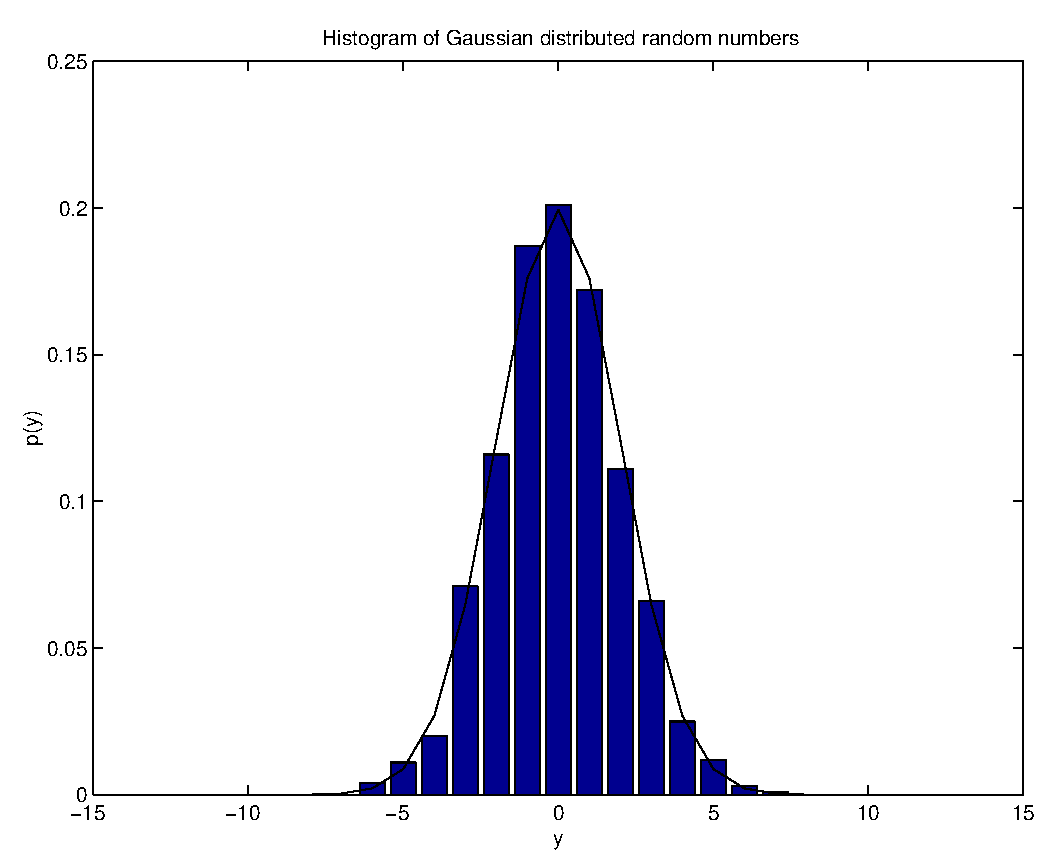
\includegraphics[width=10cm]{./Figures/f_gaussdistr.eps}
\caption{Histogram of 1000 Gaussian distributed random numbers with
mean 0 and variance 2 generated according to the Box-Muller method. 
The continuous line represents the expected Gaussian density.}
\end{figure}

Let us end this subsection by mentioned that normal distributed
random numbers can be generated in MATLAB with the help of 
the function {\sf randn}.

\section{The acceptance--rejection technique}
The acceptance--rejection technique is a method of wide 
applicability. In its original formulation it is due to 
von--Neumann. The basic idea is to sample a random number
from some known and appropriate probability distribution and to 
perform a test to determine whether or not it is acceptable for 
use or not. We follow the approach by Rubinstein 
\cite{RUBINSTEIN} but consider for simplicity only
the one--dimensional case.

Let us assume that the stochastic variable $X$ is defined on the 
interval $a \le x \le b$ and is distributed according to the
probability density $p(x)$. We write this probability distribution 
as
\begin{equation*}
p(x) = C d(x) q(x),
\end{equation*}
where $C$ is a normalization constant $C \ge 1$, $q(x)$ is also a 
probability distribution and $0 \le d(x) \le 1$. The probability 
distribution $q(x)$ is the importance function, and  we are 
supposed to know how to generate random variates distributed 
according to it.

The acceptance--rejection method works as follows. We generate two
random variates: $\xi$ is uniformly distributed on the interval
$[0,1)$ and $Y$ is distributed according to $q(y)$. Then we test
whether or nor the equality
\begin{equation*}
\xi \le d(y)
\end{equation*}
holds or not. If  the condition $\xi \le d(y)$ is satisfied, 
then $y$ is accepted as 
a random variate distributed according to $p(x)$.  If
the condition is not satisfied, the pair $(\xi,y)$ is rejected, 
and we have to try again.

It is easy to demonstrate that the above method works. Let us apply
Bayes'formula to the conditional probability $p(x|\xi \le d(y))$:
\begin{equation}
\label{A-R-BAYES}
p(x|\xi \le d(y)) = \frac{{\rm Prob}(p(\xi \le d(y)|Y=x)q(x)}
                  {{\rm Prob}(\xi \le d(y))}.
\end{equation}
It is straightforward to compute
\begin{eqnarray*}
{\rm Prob}(p(\xi \le d(y)|Y=x) &=& {\rm Prob}(\xi \le d(x)) = 
          d(x) \\
{\rm Prob}(\xi \le d(y)) & = & \int {\rm Prob}(\xi \le d(Y|Y=x)) q(x) dx \\
               &= & \int q(x) d(x)dx = \int dx \frac{p(x)}{C} = 
                   \frac{1}{C}.
\end{eqnarray*}
Inserting into (\ref{A-R-BAYES}) we obtain finally
\begin{equation*}
p(x|\xi \le d(y) = Cd(x)q(x)=p(x),
\end{equation*}
which completes the proof.

The above discussion also makes evident the role of the constant
$C$. The efficiency of the method depends on the inequality $\xi \le 
d(y)$, for independent trials the probability of success is given 
by $1/C$. $C$ represents the average number of passes which must 
be made with the algorithm in order to select a variate. It is 
clear, that in order for the method to be efficient it must be 
easy to generate random numbers according to $q(x)$ and the 
efficiency should be large, i.e., $C$ should be close to one.

In the original formulation by von--Neumann the comparison 
function was simply chosen to be the uniform distribution. If
$M$ is the maximum of $p(x)$ then we choose
\begin{eqnarray*}
q(x) & = & \frac{1}{b-a} \\
d(x) & = & \frac{p(x)}{M} \\
C & = & M(b-a).
\end{eqnarray*}
The von--Neumann algorithm then simply reads \\
1. Generate $\chi_1$ and $\chi_2$ uniformly distributed in 
    $[0,1)$. \\
2. Evaluate $Y=a+\chi_2(b-a)$. \\
3. If $\chi_1 \le p(x)/M$ then $Y$ is a variate distributed 
    according to $p(x)$. \\
4. Go to 1.

As a simple example we want to generate random numbers on $[0,1)$    
distributed according to
\begin{equation*}
p(x) = 3x^2; \;\;\; 0 \le x <1.
\end{equation*}
We choose $C=3$ and apply the von--Neumann algorithm. \\
1. Generate $\chi_1$ and $\chi_2$ uniformly distributed in 
    $[0,1)$. \\
2. Test the inequality $\chi_1 \le \chi_2^2.$     \\
3. If the equality holds we accept $\chi_2$ as a random number 
generated according to $p(x)$.

\subsubsection{Listing of the program neumann.m}
\inputlisting{./Listings/neumann.m}

The above algorithm has been implemented in MATLAB in the program
{\sf neumann.m}, which we run for $n=1000$ and $n=5000$. The 
result of the latter run can be seen in Fig. (\ref{F_NEUMANN}).
\begin{figure}
\label{F_NEUMANN}
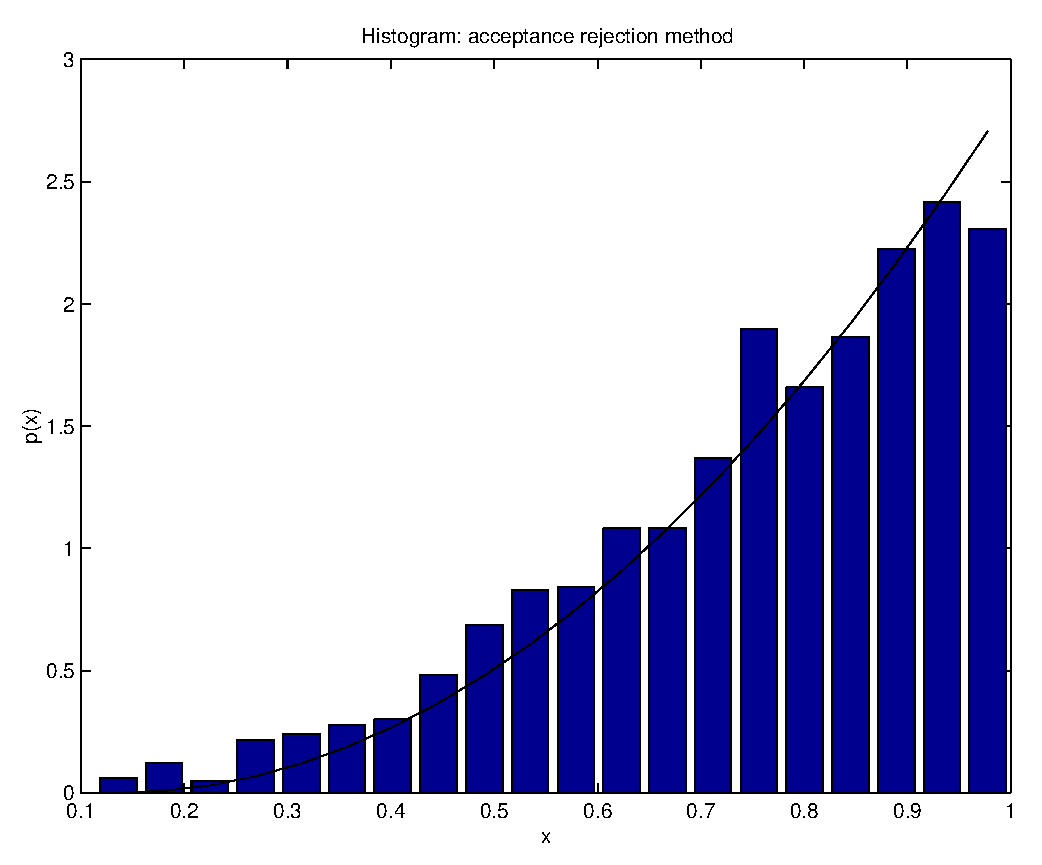
\includegraphics[width=10cm]{./Figures/f_neumann.eps}
\caption{Histogram of 5000 random numbers distributed
according to $p(x) = 3x^2$ generated with the von--Neumann
acceptance--rejection technique.
The continuous line represents the exact density $p(x)$.}
\end{figure}
In the program we count the number of successful trials. The ratio
of successful trials to the total number of drawn random pairs for 
the run shown
is 0.3328, which is in good agreement with the expected theoretical
value of $1/C=1/3$.

%\subsection{Poisson distributed random numbers}

\section{Variance reduction: Importance Sampling}
In this section we will see how the Monte--Carlo integration
algorithms can considerably be improved. The importance sampling 
technique will be our first encounter with a so--called variance 
reduction technique. We already know that the estimation of 
integrals by the Monte--Carlo method is affected with errors. The
basic idea of variance reduction techniques is to use known 
information about the problem in order to improve the efficiency 
of the simulation. Obviously, if nothing is known about the 
problem no variance reduction can be achieved. On the other 
extreme, if we have full knowledge the variance will be reduced to 
zero, and there will be no need for a simulation. It is always 
important to be aware of what is known about the system.

We consider again the problem of estimating the integral
\begin{equation}
\label{INT_VARRED}
I = \int dx f(x).
\end{equation}
The central idea of importance sampling is to select random 
variates from regions in proportion to the importance these 
regions hAve to the integral we want to evaluate, instead of 
spreading them evenly. To this end we rewrite the integral 
(\ref{INT_VARRED}) in the form
\begin{equation*}
I = \int \frac{f(x)}{p(x)} p(x) dx = \langle 
\frac{f(x)}{p(x)}\rangle,
\end{equation*}
where $X$ is a random variable with probability density $p(x)$.
$P(x)$ is called the importance sampling distribution.  Since the
integral is obviously the expectation value of the function $f(x)/p(x)$
it can be estimated using $N$ random numbers $X_i$ distributed 
according to $p(x)$
\begin{equation*}
\hat{I}_N = \frac{1}{N} \sum_{i=1}^N \frac{f(x_i)}{p(x_i)}.
\end{equation*}
The function $p(x)$ has to be chosen in such a way that the 
variance of $f(x)/p(x)$ 
\begin{equation*}
{\rm Var} = \langle (\frac{f(x)}{p(x)}-I)^2\rangle
   = \int_a^b \frac{f^2(x)}{p(x)}dx - I^2
\end{equation*}
is minimal. If $f(x)>0$ it follows from the above equation that
${\rm Var}=0$ if we choose $p(x)$ as $p(x) = f(x)/I$. 
Unfortunately, this choice implies that we know already 
the integral we want to solve. In general, the variance can 
essentially be reduced if $p(x)$ is chosen to resemble $f(x)$.

As an example we consider the integral
\begin{equation}
\label{I_MCI_IS}
I= \int_0^1 dx \exp(-x^2).
\end{equation}
In the first two columns of table (\ref{T_MCI_IS}) we show
the results of two estimates of the above integral with the 
help of the standard Monte--Carlo integration. In the third column 
we show the results of the importance sampling integration.

\begin{table}\label{T_MCI_IS}
\caption{Monte--Carlo estimates of the integral (\ref{I_MCI_IS})
using the standard method $p(x)=1$ and the importance sampling method
$p(x)=a\exp(-x)$}
\begin{center}
\begin{tabular}{llll}\hline \hline
 ~             & $p(x) =1$ & $p(x) =1$ & $p(x)=a\exp(-x)$ \\ \hline
$N$            & 1000      & 16384      & 1000           \\
$\hat{I}$            & 0.736087  & 0.74504    & 0.748340        \\
$\sigma_{\hat{I}_N}$     & 0.00131   & 0.000317   & $9.65 \times 10^{-5}$ \\
CPU time/trial (s) & 0.000660  & 0.003837   & 0.000860  \\
total CPU time (s) & 0.66      & 62.86      & 0.86  \\ 
    \hline  \hline
\end{tabular}
\end{center}
\end{table}
The simulation was performed with the help of the program
{\sf mciis.m} whose listing can be seen below.

\subsubsection{Listing of the program mciis.m}
\inputlisting{./Listings/mciis.m}

The importance sampling function is chosen to be $p(x)=a\exp(-x)$,
where the constant $a$ is chosen such that $p(x)$ is normalized
on the  unit interval. Accordingly the $N$ random numbers $X_i$
distributed according to $p(x)$ are generated with the help of the
inversion method. Since
\begin{equation*}
P(x) = \int_0^x dx' p(x') = a[1-\exp(-1)]
\end{equation*}
the exponentially distributed random numbers on the interval $[0,1)$
are generated according to
\begin{equation*}
X = - \log(1- \chi/a),
\end{equation*}
where the $\chi$ are uniformly distributed random numbers on the 
interval $[0,1)$. The generation of these random numbers is 
performed in lines x to y.

It is important to remark that although the computation time per
trial is larger in the importance sampling technique, the total CPU 
time is smaller compared to the standard Monte Carlo algorithm,
because a much smaller number of realizations is required in order
to achieve a desired accuracy (variance).

\section{Sampling of polymer configurations}
In this section we want to apply the importance sampling technique
to one simple problem of polymer physics. 
\subsection{Ideal chains}
One of the simplest idealizations of a flexible polymer chain 
consists in replacing it by a random walk on a lattice 
\cite{DE_GENNES,DOI_AND_EDWARDS}. The walk 
is a succession of steps starting from one end and reaching an 
arbitrary end point. The analogy between the random walk and the
polymer stems from the fact that one regards the realizations of 
the random walk as a possible configuration of the polymer chain.
We will start by generalizing the one--dimensional random walk
discussed in the previous chapter.

For simplicity, we consider cubic lattices in $d$ dimensions,
i.e. a square lattice for $d=2$ and a cubic lattice for $d=3$.
The stepping probability $p$ from a given site to one of its $q=2d$
neighbors  is assumed to equal $p=1/q$. The number $q$ is called
the coordination number of the lattice. The length of one step
will be $l$. The analogy between random walks and polymer chains 
is very helpful since it allows to investigate global properties 
of the polymer.

Let us assume that the random walk begins at $\vec{R}_0$ and that 
it ends after $N$ steps at $\vec{R}_N$. A typical global property
of interest in polymer physics is the end--to--end vector,
which is given by
\begin{equation*}
\vec{R} = \vec{R}_N -\vec{R}_0.
\end{equation*}
Of course, the end--to--end vector is the sum of the statistically 
independent increment vectors
\begin{equation*}
\vec{r}_i = \vec{R}_i - \vec{R}_{i-1} \;\;\; {\rm for} \;\;\; 
       i=1, \ldots, N,
\end{equation*}
i.e.,
\begin{equation*}
\vec{R} = \sum_{i=1}^N \vec{r}_i.
\end{equation*}
It is easy to generalize the results obtained previously for the 
one--dimensional random walk to $d$ dimensions. It is clear, that 
the projections of the $d$ dimensional $N$ step random walk onto 
the Cartesian axes are again one--dimensional random walks of, on 
average, $N/d$ steps. These walks are statistically independent, 
so that the probability density $p(\vec{R})$ for the displacement
of the $d$--dimensional random walk of $N$ steps is simply 
obtained as the product of $d$ one--dimensional random walks of $N/d$
steps each
\begin{equation*}
P(\vec{R},N) = P(R_1,N/d) P(R_2,N/d) \cdots P(R_d,N/d),
\end{equation*}
which inserting the Gaussian density for $P(R_1,N/d)$ from Chap. 2 Eq. 
(\ref{MULTI_GAUSS}) is immediately found to be a $d$--dimensional Gaussian 
probability density
\begin{equation*}
P(\vec{R},N) = \left(3/2 \pi Nl^2 \right)^{(3/2)} 
              \exp\left( - \frac{3\vec{R}^2}{2Nl^2}\right).
\end{equation*}
Obviously, the mean of the end--to--end distance is zero. The mean
squared end--to--end distance, i.e. the variance of $\vec{R}$, 
is (see Chap. 2) 
\begin{equation}
\label{RW_R2}
\langle \vec{R}^2 \rangle = N l^2,
\end{equation}
which is again linear in $N$.

It is also instructive to look at the fluctuations of $\vec{R}^2$,
\begin{equation*}
\Delta_R = \frac{\sqrt{\langle \vec{R}^4 \rangle - 
                   \langle \vec{R}^2\rangle^2}}
             {\langle \vec{R}^2\rangle}
             = \sqrt{\frac{2}{3}}.
\end{equation*}
We immediately recognize that the variance $\Delta_R$ does not 
decrease with increasing system size. Usually, in statistical physics
fluctuations decrease with increasing number of degrees of freedom.
Accordingly, the difference between expectation values and the 
true ensemble average
scales with $1/\sqrt{N}$. Such a property is called
self--averaging. It follows from the above discussion that  
Random walks do not have the self--averaging property.

At this stage it might be appropriate to introduce the concept of 
universality, which allows the classification of the critical 
behaviour of a large variety of systems in classes with the same 
universality. The simple properties of the random walk allow the 
introduction of the Gaussian universality class. Denoting by
$R = \sqrt{\langle \vec{R}^2\rangle}$ the size of the polymer, we 
can write  Eq. (\ref{RW_R2}) in the form
\begin{equation*}
R = N^{\nu}l,
\end{equation*}
where for the simple random walk $\nu = 1/2$ and $R$ is independent of 
the dimensionality of the lattice. As we will see soon, for other 
random walks the critical exponent $\nu$ strongly depends on the 
dimension of the lattice.

Since we want to sample with the help of the following program
configurations of ideal polymers it is important to consider how 
many configurations are possible. To this end we compute the 
number $Z_N$ of distinct random walks. Since each lattice site 
has $q$ neighbors,
the number of distinct possibilities at each step is $q$ and the 
total number of configurations is
\begin{equation}
\label{Z_NRW}
Z_N = q^N.
\end{equation}

In order to demonstrate the above theoretical results we want to 
simulate now a random walk on a two dimensional lattice.
The listing can be seen below and will be discussed soon.

\subsubsection{Listing of the program random walk}
\inputlisting{./Listings/rw_2d.m}

Figuren: Konfigurationen !!!! \\

Figuren: end-to-end !!!!\\

Figuren/Tabelle: kritischer Exponent !!!! \\

Diskussion \\

\subsection{Real chains}
In Fig. () we see that the realizations of the random walk, i.e. 
the polymer chains intersect themselves. This is of course an 
unphysical behaviour since real polymer chains do not intersect.
In order to simulate real chains on a lattice we still can 
represent  the polymer as a random walk, but now the walk can not 
intersect itself. Such random walks are called self--avoiding 
random walks (SAW). In other words the SAW has the constraint that 
the walker cannot return to sites he already visited. As a natural 
consequence SAWs are more extended then the usual random walks. Of 
course, also the universal properties of the SAW are different 
from those of the Gaussian random walk. In particular the exponent
$\nu$ strongly depends on the dimension of the lattice. It is 
clear that in $d=1$ a SAW is simply a rigid rod and we have 
$\nu=1$. For increasing dimension of the lattice $\nu$ 
decreases as the self--avoiding constraint becomes less important. 
For large dimensions the difference between random walk and SAW 
vanishes. In fact for the critical dimension $d_c =4$ random walk 
and SAW have the same universal properties. 

In general it is not 
possible to evaluate the critical exponent $\nu$ analytically for the 
SAW. This is possible only for $d=1,d=2$ and $d \ge4$. However, a 
simple mean field theory, the Flory theory, makes the following 
predictions
\begin{equation*}
\nu = \left\{ \begin{array}{cl}
               3/(2+d) & \;\;\; {\rm for} \;\;\; 1 \le d \le 4, \\
               1/2     & \;\;\; {\rm for} \;\;\; d\ge 4.
\end{array}
       \right.
\end{equation*}
As we will see this theoretical predictions agree well with the 
stochastic simulations (!!!!!).

The total number of self--avoiding random walks of $N$  steps has 
(for large $N$) the following asymptotic form
\begin{equation*}
Z_N = {\rm constant} \quad N^{\gamma-1} q_{\rm eff}^N.
\end{equation*}
The second factor in the above scaling law reminds us of the expression
(\ref{Z_NRW})  which holds for ideal random walks. The effective 
coordination number is smaller then the coordination number $q$, 
e.g. in 3 dimensions we have $q=6$ and $q_{\rm eff}=4.68$. The first factor
$N^{\gamma -1}$  is called the enhancement factor. The universal
exponent $\gamma$ depends on the dimension of the lattice
\begin{equation*}
\gamma \approx \left\{ \begin{array}{cl}
                        7/6 & {\rm for} \;\;\; d=3 \\
                        4/3 & {\rm for} \;\;\; d=2.
                       \end{array}
               \right.
\end{equation*}
Note that for $d=1$ we have $Z_N = 2$, independently of $N$. 
Hence, $q_{\rm eff} = 1$ and $\gamma =1$.

As an application of the sampling techniques we have learned in 
this chapter we address the problem of generating 
configurations of real polymer chains on a lattice, or in other 
words we want to generate realizations of SAW on the computer.

DISKUSSION VON E(R2) SAW !!!!!!!!!!!!!

\subsubsection{Simple sampling}
The simplest algorithm to generate chains of  length $N$ is the 
following one. We start at the origin. The first step is, of 
course,  taken randomly from the $q$ adjacent sites. The following 
steps are taken from the remaining $q_0=q-1$ possible directions, 
because a direct backfolding is forbidden. Of course, the SAW 
condition is also violated whenever the chosen lattice site is 
already taken. In fact, the self--avoiding walk has an infinite
memory. In such cases the attempted walk is terminated and 
discarded and we have to start with a new chain. In this way we 
automatically fulfill the condition that all walks  of equal 
length have the same probability. All sampled configurations are 
statistically independent and hence the standard error analysis 
is possible. It is instructive to estimate that the success rate
$s_N$, i.e., the fraction of walks that will continue successfully 
for $N$ steps, is of the order
\begin{equation*}
s_N = \frac{Z_N(SAW)}{q(q-1)^N} \approx
      \frac{N^{\gamma -1} q_{\rm eff}^N}{q(q-1)^N}
       = \left( \frac{q_{\rm eff}^N}{q-1}\right) 
         \left( \frac{q-1}{q} \right) N^{\gamma -1},
\end{equation*}
which for large $N$ decreases exponentially as
\begin{equation*}
s_N \approx \exp(-N \mu),
\end{equation*}
with $\mu=\ln[(q-1)/q_{\rm eff}]$. 
On a two--dimesnional lattice $1/\mu = 7.75$, on a 3d lattice
$1/\mu = 15.4$ (CHECK!!!!!!!!!!!!!!!!). Because of this exponential 
decrease it is very  difficult to generate very long chains with 
the simple sampling algorithm. This problem is called the 
"attrition problem".

FIGUREN ZUM ATTRITION PROBLEM !!!!!!!!!

\subsubsection{Biased sampling}
To overcome the attrition problem it is necessary to exploit 
biased sampling techniques. One such technique is the "inversely
restricted sampling" of Rosenbluth and Rosenbluth \cite{ROSENBLUTH}. 
The idea is to
associate each SAW of $N$ steps with appropriately chosen weighting 
factors. 

We consider a SAW of $i$ steps on a lattice with the coordination 
number $q$. In order to sample the next step we have to check  
which of the $q_0 = q-1$ neighboring sites is empty. Essentially,
we have two possibilities:

1. If $k$ ($q_0 \ge k >0$) sites are empty we choose the possible 
steps with equal probability $1/k$.

2. If there is no empty site ($k=0$) we terminate the walk and 
start from the beginning.

It is clear that each $N$ step walk has the probability
\begin{equation*}
P_N(\{ \vec{r}_i \}) = \prod_{i=1}^N (k_i)^{-1}
\end{equation*}
and hence dense configurations are more probable. Thus this 
obvious procedure of choosing only among those  sites that do not 
violate the SAW condition does not give equal statistical weights
to the generated configurations. But since we have seen that these 
weight can be calculated we can compensate this bias by weighting 
each chain in the sample by the factor
\begin{equation*}
W_N(\{ \vec{r}_i \}) =  \prod_{i=1}^N \frac{k_i}{q_0}.
\end{equation*}
Since, $W_N P_N = q_0^{-N}$ the biased sampling procedure samples 
exactly the same configuration space as simple sampling.

The correct way to estimate $\langle \vec{R}^2 \rangle$ is
\begin{equation*}
\langle \vec{R}^2 \rangle = \frac{\sum_{l=1}^M W_{N,l} R^2_{N,l}}
                               {\sum_{l=1}^M W_{N,l}},
\end{equation*}
where the sum is over all realizations.

In order to compare the two sampling techniques we have written a 
program {\sf RW\_2D\_sa2.m} which by specifying an input parameter
draws configurations of real chains on a two--dimensional squared lattice 
with the simple sampling 
technique or with the biased (importance) sampling technique.



\subsubsection{Listing of the program {\sf RW\_2D\_sa2.m}}
\inputlisting{./Listings/RW_2D_sa2.m}

Let us comment on the program. BLA BLA BLA !!!!!!!!!

In table (\ref{T_SAW}) we see some results of the simulations.
\begin{table}
\label{T_SAW}
\caption{Values of $<\vec{R}^2>$ as functions of $N$, 
for the two--dimensional random walk with biased sampling.}
\begin{center}
\begin{tabular}{rrrr} \hline \hline
$N$ & Memory & No. chains & $<\vec{R}^2>$ \\ \hline
10  & 0        & 1000     &    123 \\
10  & $\infty$ & 1000     & 123 \\
20  & 0        & 1000     & 123   \\
20  & $\infty$ & 1000     & 123 \\
30  & 0        & 1000     & 123 \\ 
30  & $\infty$ & 1000     & 123 \\ \hline \hline
\end{tabular}
\end{center}
\end{table}


In table (\ref{T_SAW_NU}) we show some estimated values of 
the critical exponent $\mu$.
\begin{table}
\label{T_SAW_NU}
\caption{The critical exponent $\nu$.}
\begin{center}
\begin{tabular}{lll}\hline \hline
Memory   & $\nu$ & $\nu_{\rm Theory}$ \\ \hline
0        & 123   & 1/2 (RW)  \\
$\infty$ & 123   & 3/4 (Flory) \\
\hline \hline
\end{tabular}
\end{center}
\end{table}

IRGENDEIN VERGLEICH ZWISCHEN SIMPLE UND IMPORTANCE SAMPLING !!!!!


FIGUREN: REALISIERUNGEN, SKALENVERHALTEN, End-TO-END ABSTAND,
FEHLER, USW.


%%%%%%%%%%%%%%%%%%%%%%%%%%%%%%%%%%%%%%%%%%%%%%%%%%%%
%%%%%%%%%%%%%%%%%%%%%%%%%%%%%%%%%%%%%%%%%%%%%%%%%%%%%
%%%%%%%%%%%%%%%%%%%%%%%%%%%%%%%%%%%%%%%%%%%%%%%%%%%%%
%%%%%%%%%%%%%%%%%%%%%%%%%%%%%%%%%%%%%%%%%%%%%%%%%%%%%
%%%%%%%%%%%%%%%%%%%%%%%%%%%%%%%%%%%%%%%%%%%%%%%%%%%%%
%%%%%%%%%%%%%%%%%%%%%%%%%%%%%%%%%%%%%%%%%%%%%%%%%%%%%
%%%%%%%%%%%%%%%%%%%%%%%%%%%%%%%%%%%%%%%%%%%%%%%%%%%%%
\chapter{Stochastische Prozesse}
Master-Gleichungen

\chapter{Monte Carlo Methoden in der statistischen Mechanik}
Metropolis; Ising; Finite-Size Effects; Random Walks; SAW (?)
Simulated annealing; travelling salesman;

\chapter{Non-equilibrium MC}
Chemische Reaktionen, Diffusion; Reaktions-Diffusion, Turbulenz.

\chapter{Brownsche Dynamik Simulationen}
Omega-entwicklung; SDE;


\chapter{Rest}
stochastische Resonanzen; Muster Erkennung; random Walks;

\chapter{Stochastische Wellenfunktionsmethoden}
